% docs/Latex/Result.tex
% Results of training the three design proposals catalogued in arc.tex (2026-09-29/30 run, TASK-20260929-016).
% Only results are reported; every number comes from raw result JSONs under output/arc_proposals/ (branch
% claude/arc-design-proposals-training-3a3ac9, PR #12). Figures are made by scripts/make_result_plots.py from those files.
\documentclass[11pt]{article}
\emergencystretch=3em

\usepackage[margin=2.5cm]{geometry}
\usepackage{booktabs}
\usepackage{graphicx}
\usepackage{array}
\usepackage{xcolor}
\usepackage{hyperref}
\usepackage{caption}
\usepackage{amsmath}
\usepackage{parskip}

\graphicspath{{figures/}}
\newcommand{\srcpath}[1]{\texttt{\small #1}}

\title{Training the three arc.tex design proposals: what we ran and what came out}
\author{}
\date{Run of 2026-09-29/30}

\begin{document}
\maketitle

\section{What this is}

\texttt{arc.tex} lists three design proposals. We trained and tested them on a local RTX 3060 Ti and on Kaggle T4 GPUs, including a few derivative models and
parameter adjustments made after looking at medium-scale results. This file only reports what was run and what came out. Result files live under \srcpath{output/arc\_proposals/} on the PR branch. Scripts (all in \srcpath{scripts/}):
\begin{itemize}\itemsep0pt
\item \srcpath{run\_structure\_input\_planning.py}, \srcpath{run\_structure\_input\_prediction.py},
\item \srcpath{analyze\_structure\_route\_selection.py}
\item \srcpath{run\_actor\_critic\_litmus.py}, \srcpath{run\_action\_reward\_model.py}
\item \srcpath{run\_latency\_sweep2.py}, \srcpath{make\_result\_plots.py} (figures and numbers in this file)
\end{itemize}

Mapping used between the proposals and the sections of \texttt{arc.tex}:
\begin{itemize}
\item \textbf{Structure-as-input world model} = \texttt{phys\_feat} and \texttt{skip\_feat0}: a known (possibly wrong) formula is given to the learned potential as an \emph{input feature} (arc.tex \S4).
\item \textbf{Actor-critic and the \texttt{oracle\_act} litmus} = replace REINFORCE by an actor-critic learner and ask whether the leaked positive control \texttt{oracle\_act} now clearly beats \texttt{base} (arc.tex \S2.5, \S2.4, \S2.8).
\item \textbf{ChunkPPO with $\delta>0$} = chunk-level PPO with a latency of $\delta$ ticks, arms \texttt{ignore}, \texttt{augment}, \texttt{wm}, \texttt{wm\_passive}, \texttt{oracle} (arc.tex \S3).
\end{itemize}

\paragraph{Summary.}
\begin{center}
\footnotesize
\begin{tabular}{@{}p{2.6cm}p{12.4cm}@{}}
\toprule
Proposal & Outcome \\
\midrule
Structure-as-input & Works on the pendulum (planning return $-204$ vs.\ $-271$ without the feature; ceiling $-196$), but generic unbounded features ($|q|$, $q^3$, $q^4$) do just as well, so the gain comes from an extrapolating input basis, not from the physics. A wrong formula used as a hard term is much worse. \\
Actor-critic + \texttt{oracle\_act} & The litmus passes: \texttt{oracle\_act} beats \texttt{base} by $+1.0$ (12.8k episodes) and $+1.8$ (49.9k episodes); REINFORCE showed $+0.07$. A noop-future world model adds nothing beyond random features. A learned action-reward model gets part of the leaked gain at 12.8k episodes (about a quarter) and a small, not significant part at 49.9k. \\
ChunkPPO $\delta>0$ & No reproducible advantage of the forecast arms over \texttt{augment}/\texttt{ignore}. The one significant gap (intercept, $\delta=2$) disappears with a second learner configuration; all gaps close at 10M ticks; on \texttt{pendulum\_goal} the forecast arms are slightly worse. \\
\bottomrule
\end{tabular}
\end{center}

\section{Structure-as-input world model}

\subsection{What we did}
Same network, data, optimiser and step count in every arm; only the scalar feature handed to the learned potential $V$ changed.
The learned model is a port-Hamiltonian network $\dot x=(J-R)\nabla H$ with $H=|p|^2/2+\mathrm{MLP}(q,\,\text{feature}(q))$ (feature route), or the feature added
directly to $H$ with a learned scale (\emph{skip}, gate initialised at 0 or 1), or added as a fixed term (\emph{hard}). The feature variants were:
the proposal's small-angle preset $q^2/2$; a rescaled $1.5q^2$; the true potential $-\cos q$ (an oracle, upper bound only); generic physics-free bases ($|q|$, $q^3/3$, $q^4/4$, the pair $[q^2/2,q^4/4]$);
bounded oscillatory features ($\sin(5q+0.7)$, $-\cos 2q$); a zero feature (same architecture, no information); and no feature at all (\texttt{hn}); plus a plain MLP.

Two testbeds:
\begin{itemize}
\item \textbf{Planning}: torque-limited pendulum swing-up ($|u|\le 0.7$, start hanging, goal upright). Offline data: $N\in\{8,32,128\}$ short trajectories from initial angles $|\theta_0|<1.5$ with random piecewise-constant torques, 2\% observation noise, 2000 Adam steps, 10-step open-loop loss.
The learned model is used inside a CEM model-predictive controller (3 iterations $\times$ 256 samples, horizon 60, replanning every step); the environment is stepped with the true dynamics. Score = return over 24 episodes; 6--12 seeds per cell.
\item \textbf{Rollout prediction} on four tasks (Kepler with an unmodelled perturbation, Kepler with a wrong $\mu$ preset, falling body with quadratic drag, pendulum), $N=64$ trajectories, 2\% noise, 3000 steps, 5 seeds; metric = mean normalised RMSE over a 200--250-step open-loop rollout on held-out initial conditions inside the training range (ID) and outside it (OOD).
\end{itemize}

\subsection{Results: planning}
\begin{figure}[h]
\centering
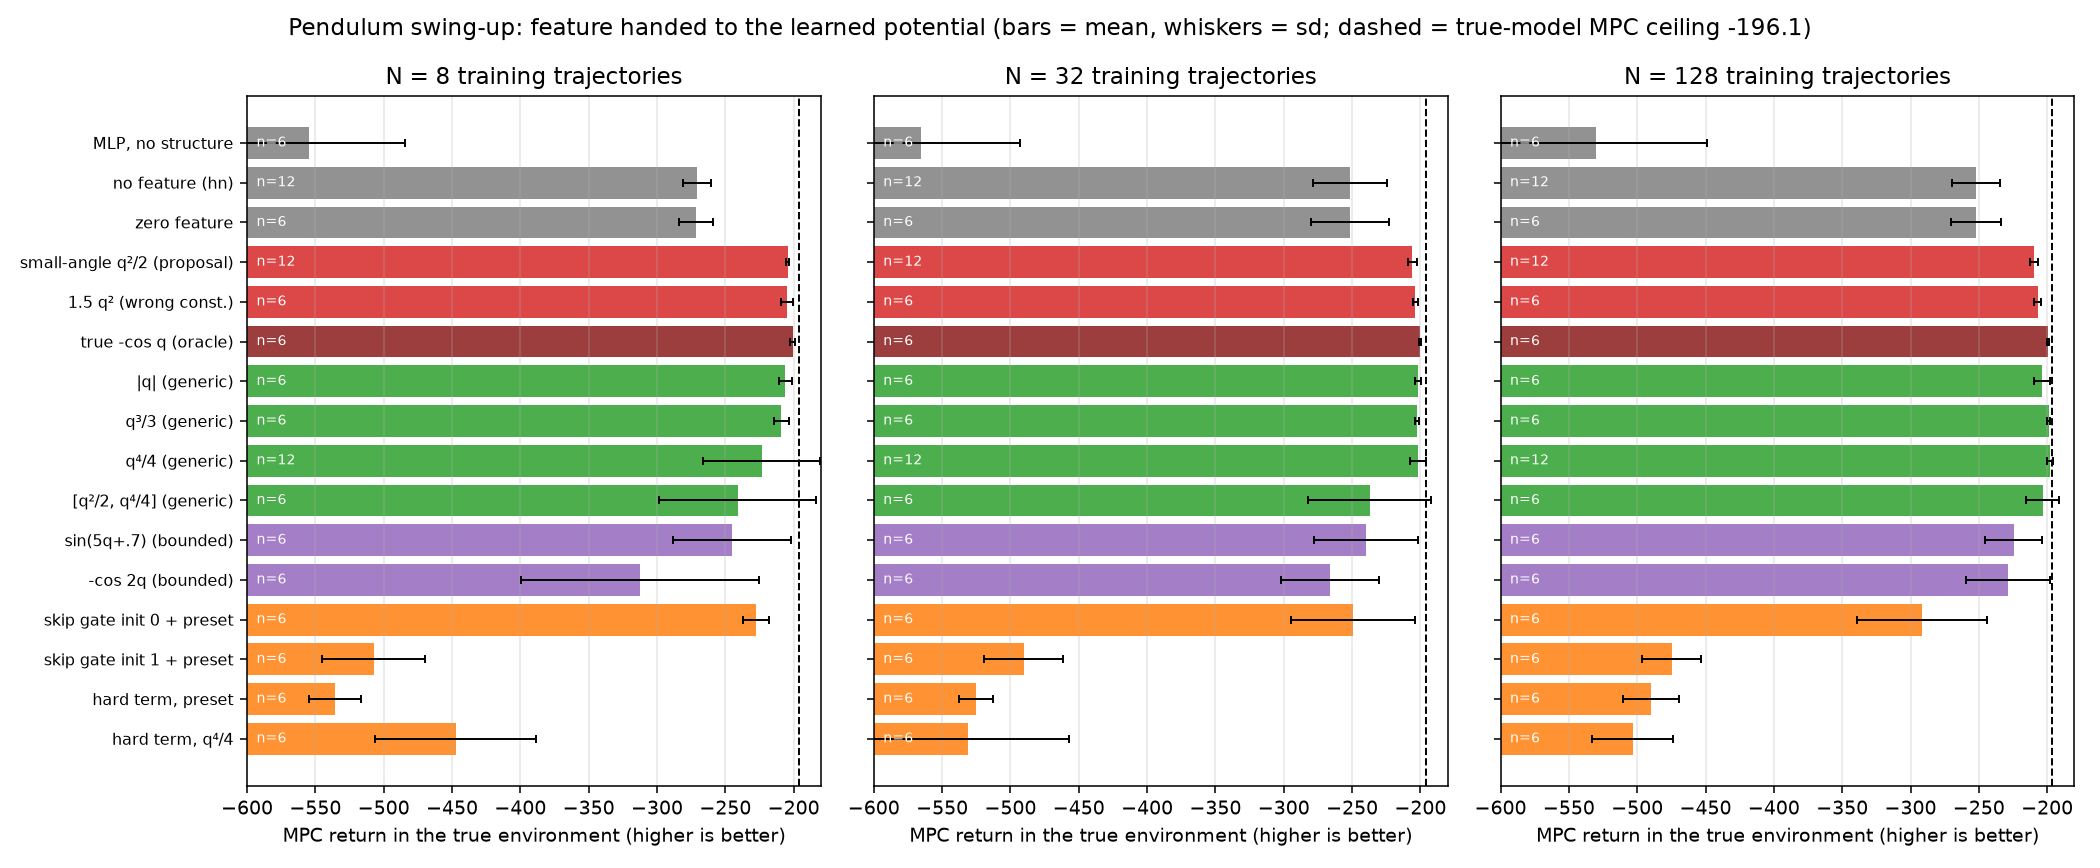
\includegraphics[width=\textwidth]{res_structure_planning.png}
\caption{Pendulum swing-up MPC return in the true environment for each feature given to the learned potential, at three data sizes (mean $\pm$ sd over seeds; $n$ printed in the bars; dashed line = true-model MPC ceiling $-196.1$). Source: \srcpath{output/arc\_proposals/structure\_input/planning\{,2\}/}.}
\end{figure}

\begin{table}[h]
\centering\small
\caption{Selected planning results (mean $\pm$ sd; 12 seeds for hn, small-angle and $q^4/4$, 6 otherwise). Same source as the figure.}
\begin{tabular}{lrrr}
\toprule
feature & $N=8$ & $N=32$ & $N=128$ \\
\midrule
MLP (no structure) & $-555\pm70$ & $-566\pm73$ & $-530\pm82$ \\
none (hn) & $-270.5\pm10$ & $-251.4\pm27$ & $-252.0\pm18$ \\
zero feature & $-271.3\pm12$ & $-251.5\pm29$ & $-252.0\pm19$ \\
small-angle $q^2/2$ (proposal) & $\mathbf{-204.3\pm1.0}$ & $-206.0\pm3.4$ & $-209.4\pm2.8$ \\
true $-\cos q$ (oracle) & $-200.8\pm1.6$ & $-200.5\pm0.8$ & $-199.4\pm0.8$ \\
$|q|$ (generic) & $-206.2\pm4.8$ & $-201.5\pm2.3$ & $-203.7\pm5.8$ \\
$q^3/3$ (generic) & $-209.0\pm5.6$ & $-202.4\pm1.4$ & $-198.7\pm1.1$ \\
$q^4/4$ (generic) & $-223\pm43$ & $-201.6\pm5.9$ & $-197.8\pm2.2$ \\
$\sin(5q+0.7)$ (bounded) & $-245\pm43$ & $-240\pm38$ & $-225\pm21$ \\
$-\cos 2q$ (bounded) & $-312\pm87$ & $-266\pm36$ & $-229\pm31$ \\
skip gate init 0 + preset & $-227.5\pm9$ & $-249\pm45$ & $-292\pm48$ \\
skip gate init 1 + preset & $-507\pm38$ & $-490\pm29$ & $-475\pm22$ \\
hard term, preset & $-536\pm19$ & $-525\pm13$ & $-490\pm20$ \\
\bottomrule
\end{tabular}
\end{table}

What we read from this:
\begin{itemize}
\item The proposal's feature route gives about 65 return units over no feature at $N=8$, and stays within 3--10 units of the true-model ceiling at every data size.
\item The zero feature is identical to no feature, so the extra input dimension by itself does nothing.
\item The same gain is obtained by $|q|$ and $q^3$ (no physical content) and by $q^4$ from $N=32$ on. Bounded oscillatory features do not help. So the effect is an \emph{unbounded, monotone} input that lets the network extrapolate to the upright region, which the data never visit; the physics preset is the most reliable member of that family at $N=8$ (sd 1 vs.\ 43 for $q^4$).
\item Using the same wrong formula as a fixed term or a skip connection starting open is far worse ($-450$ to $-540$); a skip starting closed is in between and gets worse with more data.
\end{itemize}

\subsection{Results: rollout prediction}
\begin{figure}[h]
\centering
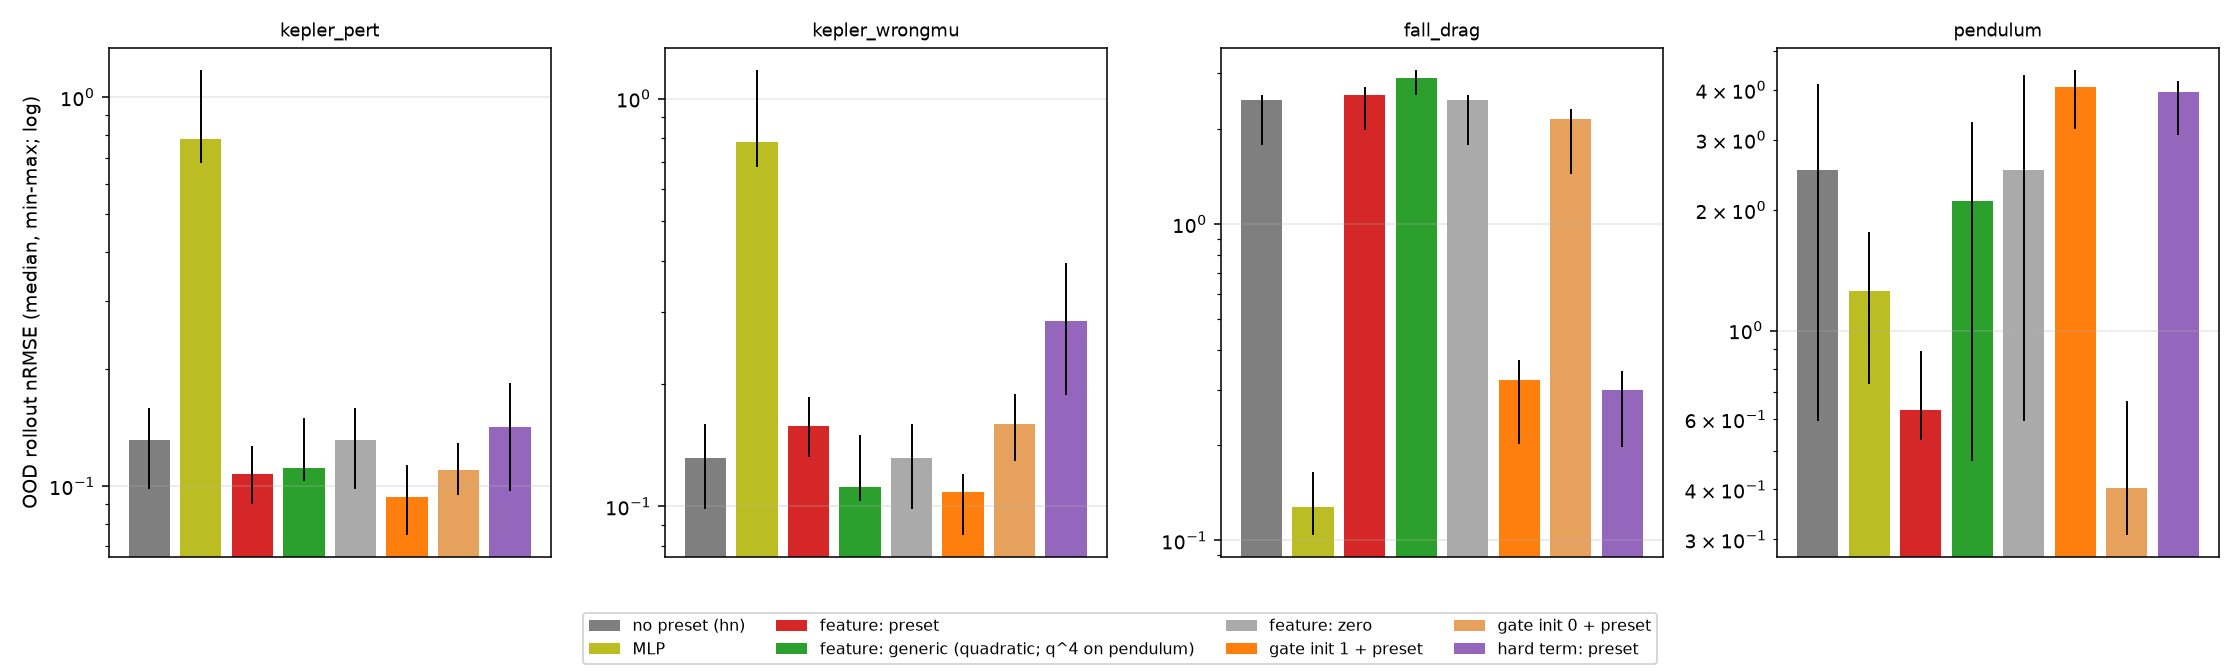
\includegraphics[width=\textwidth]{res_structure_prediction.png}
\caption{Out-of-distribution rollout error (median over 5 seeds, whiskers = min--max, log scale) per task and route. ``Generic'' is a quadratic on the Kepler and falling-body tasks and $q^4/4$ on the pendulum. Source: \srcpath{output/arc\_proposals/structure\_input/prediction\{,2\}/}.}
\end{figure}

\begin{table}[h]
\centering\small
\caption{Median mean-nRMSE over 5 seeds, ID / OOD (lower is better).}
\begin{tabular}{lrrrr}
\toprule
route & Kepler pert. & Kepler wrong $\mu$ & falling + drag & pendulum \\
\midrule
no preset (hn) & .140 / .132 & .140 / .132 & .467 / 2.47 & .013 / 2.52 \\
feature: preset & .149 / .107 & .164 / .158 & .672 / 2.56 & .013 / \textbf{.634} \\
feature: generic & .139 / .111 & -- & 1.28 / 2.90 & .015 / 2.11 \\
feature: zero & .140 / .132 & .140 / .132 & .467 / 2.47 & .013 / 2.52 \\
gate init 0 + preset & .150 / .110 & .158 / .160 & .512 / 2.15 & .013 / \textbf{.404} \\
gate init 1 + preset (OOD only) & .093 & .109 & .321 & 4.08 \\
hard term: preset & .187 / .142 & .331 / .285 & \textbf{.149 / .298} & .037 / 3.95 \\
\bottomrule
\end{tabular}
\end{table}

On Kepler the feature route is within noise of \texttt{hn} (which already has the Hamiltonian prior) and a generic quadratic does as well as the Newton preset. On the falling body the \emph{hard} term wins, because the preset (gravity) is exactly right for the part it covers. On the pendulum the feature route (and the closed-gate skip) is what fixes extrapolation. No single route is best on all four tasks.

\subsection{Derivative: choosing the route by held-out in-distribution error}
For each task and seed we picked among \{hn, feature, closed-gate skip, open-gate skip, hard term\} using only the ID error, then read off the OOD error of the chosen route (no new training; reuse of the runs above).

\begin{table}[h]
\centering\small
\caption{Median OOD nRMSE over seeds for each fixed route and for the ID-selected route.}
\begin{tabular}{lrrrrrrr}
\toprule
task & hn & feature & skip0 & skip1 & hard & \textbf{selected} & hindsight best \\
\midrule
falling + drag & 2.473 & 2.564 & 2.148 & 0.321 & 0.298 & \textbf{0.321} & 0.298 \\
Kepler pert. & 0.132 & 0.107 & 0.110 & 0.093 & 0.142 & \textbf{0.093} & 0.093 \\
Kepler wrong $\mu$ & 0.132 & 0.158 & 0.160 & 0.109 & 0.285 & \textbf{0.110} & 0.109 \\
pendulum & 2.522 & 0.634 & 0.404 & 4.082 & 3.949 & \textbf{2.389} & 0.404 \\
\midrule
geometric mean & 0.573 & 0.407 & 0.351 & 0.340 & 0.467 & \textbf{0.298} & 0.187 \\
\bottomrule
\end{tabular}
\end{table}
Selecting by ID error beats every fixed route on average, but on the pendulum all routes have ID error $\approx0.013$, so the OOD lock-in of a wrong preset is invisible to it (it picks \texttt{hn} in 3 of 5 seeds; OOD 2.39 vs.\ 0.40 for the best route).

\section{Actor-critic learner and the \texttt{oracle\_act} litmus}

\subsection{What we did}
\paragraph{Learner.} New actor-critic code (\srcpath{src/pipeline/candidate\_actor\_critic.py}); the REINFORCE code is untouched. PPO with clipped ratio (0.2), GAE($\lambda=0.95$, $\gamma=0.99$), entropy bonus 0.01, value coefficient 0.5, 4 epochs $\times$ 4 minibatches per update, 64 episodes of $T=250$ per update, linear lr decay, AdamW. The critic is a small MLP (2$\times$128, tanh) on the 39-d observation summary plus $t/T$ and is identical in every arm, so extra features never reach it.
The actor is the same \texttt{transformer\_branch} as in the REINFORCE study ($d=256$, 277K parameters) on Craftax-Classic through \texttt{CraftaxFutureAdapter}. Budgets: 200 updates = 12{,}800 episodes (the REINFORCE budget diagnostic) and 780 updates = 49{,}920 episodes. Metric: mean return of 256 evaluation episodes of the final sampled policy; seeds are separate training runs. lr was 1e-3 unless stated.

\paragraph{Arms.} \texttt{base}: 78 anticipation slots filled with zeros. \texttt{oracle\_act}: slots hold the \emph{true} one-step reward of each of the 17 actions (simulator branching at policy time; leaked positive control). \texttt{oracle}: true simulated noop future. \texttt{wm\_full}: predictions of the trained passive world model from the full observation. \texttt{wm\_untrain}: same network, random initialisation (control). Reference policies: a random policy and ``argmax of the leaked one-step reward'' (\emph{greedy-1}), which scores mean return 3.17 (crafter score 2.76).

\subsection{Litmus test}
\begin{figure}[h]
\centering
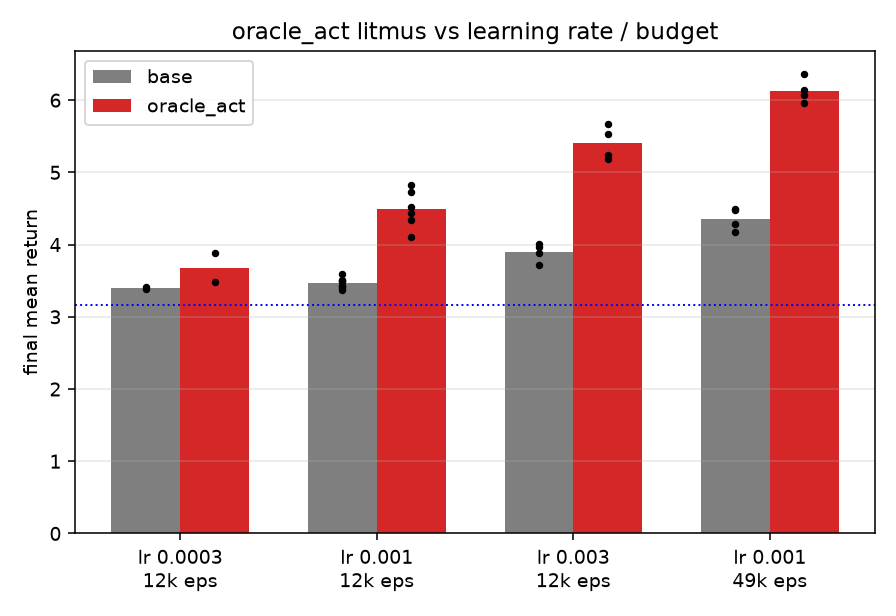
\includegraphics[width=0.62\textwidth]{res_ac_lr.png}
\caption{\texttt{base} vs.\ \texttt{oracle\_act} for different learning rates and budgets (bars = mean, dots = seeds; dotted line = greedy-1 reference 3.17). Source: \srcpath{output/arc\_proposals/ac\_litmus\_v*/}, \srcpath{ac\_long*/}.}
\end{figure}

\begin{table}[h]
\centering\small
\caption{Final mean return, mean $\pm$ sd over seeds. REINFORCE numbers are the values quoted in arc.tex \S2.5 (12{,}800 episodes, last-3-eval return).}
\begin{tabular}{lrrrr}
\toprule
learner, budget & \texttt{base} & \texttt{oracle\_act} & gap & seeds \\
\midrule
REINFORCE, 12.8k episodes & $3.25\pm0.14$ & $3.32\pm0.06$ & $+0.07$ & 4 \\
actor-critic lr $3\cdot10^{-4}$, 12.8k & $3.40\pm0.03$ & $3.68\pm0.28$ & $+0.28$ (p=0.38) & 2 \\
\textbf{actor-critic lr $10^{-3}$, 12.8k} & $3.47\pm0.07$ & $4.49\pm0.26$ & $+1.03$ (p=$1\cdot10^{-4}$) & 8 / 6 \\
actor-critic lr $3\cdot10^{-3}$, 12.8k & $3.90\pm0.13$ & $5.41\pm0.23$ & $+1.51$ (p=$1\cdot10^{-4}$) & 4 \\
\textbf{actor-critic lr $10^{-3}$, 49.9k} & $4.36\pm0.16$ & $6.13\pm0.17$ & $+1.78$ (p=$5\cdot10^{-6}$) & 4 \\
\bottomrule
\end{tabular}
\end{table}
At lr $10^{-3}$ every \texttt{oracle\_act} seed is above every \texttt{base} seed (12.8k: min 4.10 vs.\ max 3.59; 49.9k: min 5.96 vs.\ max 4.50). Crafter score at 49.9k: 8.2 (\texttt{oracle\_act}) vs.\ 4.8 (\texttt{base}). \texttt{oracle\_act} is also well above the greedy-1 reference (3.17), so the learner uses the leaked signal beyond greedy use. The learner improves \texttt{base} itself with more episodes (3.47 $\to$ 4.36). Greedy-argmax evaluation is much lower than sampled evaluation for \texttt{base} (0.95 vs.\ 3.47 at 12.8k).

\subsection{Does a passive (noop) world model help?}
\begin{figure}[h]
\centering
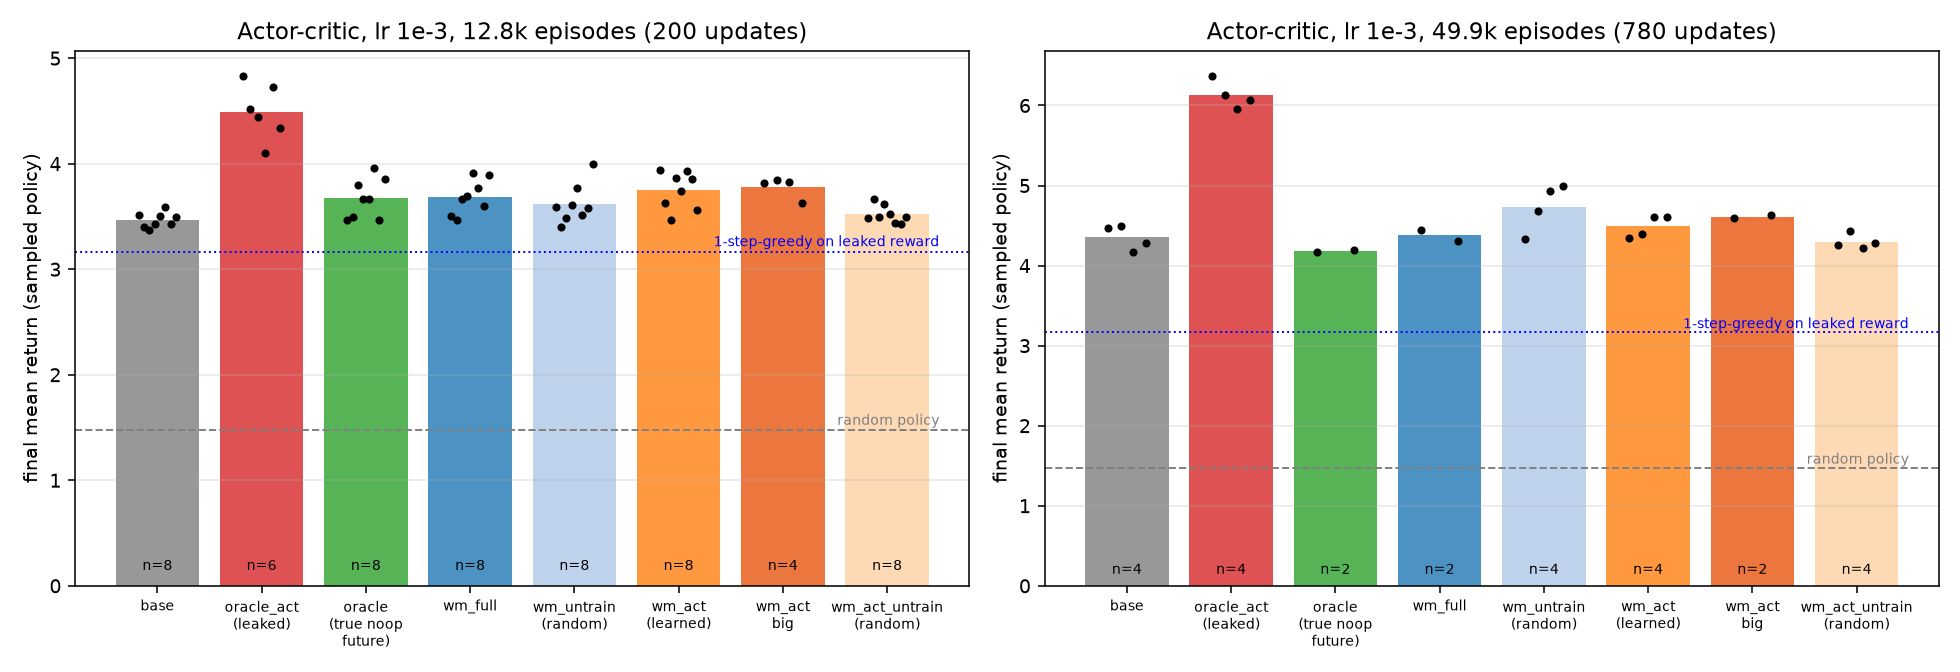
\includegraphics[width=\textwidth]{res_ac_final_returns.png}
\caption{Final mean return of all actor-critic arms at lr $10^{-3}$ (dots = seeds; dotted blue = greedy-1 reference; dashed grey = random policy). \texttt{wm\_act} arms are the learned action-reward model described below. Source: \srcpath{output/arc\_proposals/ac\_*/}.}
\end{figure}

\begin{table}[h]
\centering\small
\caption{Noop-anticipation arms, lr $10^{-3}$. $\Delta$ is relative to \texttt{base}; Welch p-values in brackets.}
\begin{tabular}{lrrrr}
\toprule
arm & 12.8k episodes & $\Delta$ & 49.9k episodes & $\Delta$ \\
\midrule
\texttt{base} & $3.47\pm0.07$ (n=8) & -- & $4.36\pm0.16$ (n=4) & -- \\
\texttt{wm\_untrain} (random) & $3.62\pm0.19$ (8) & $+0.15$ (.06) & $4.73\pm0.30$ (4) & $+0.38$ (.08) \\
\texttt{wm\_full} (trained) & $3.69\pm0.16$ (8) & $+0.22$ (.006) & $4.38\pm0.10$ (2) & $+0.02$ (.86) \\
\texttt{oracle} (true noop future) & $3.67\pm0.19$ (8) & $+0.20$ (.02) & $4.18\pm0.02$ (2) & $-0.17$ (.11) \\
\texttt{oracle\_act} (leaked) & $4.49\pm0.26$ (6) & $+1.03$ & $6.13\pm0.17$ (4) & $+1.78$ \\
\bottomrule
\end{tabular}
\end{table}
At 12.8k episodes the trained WM and even the true noop future are only $+0.2$ above \texttt{base}, and $\texttt{wm\_full}-\texttt{wm\_untrain}=+0.07$ (p=0.44), $\texttt{oracle}-\texttt{wm\_untrain}=+0.05$ (p=0.58). At 49.9k episodes the trained WM and the true noop future are no better than \texttt{base}, while the random-initialisation control is the highest of the three.

\begin{figure}[h]
\centering
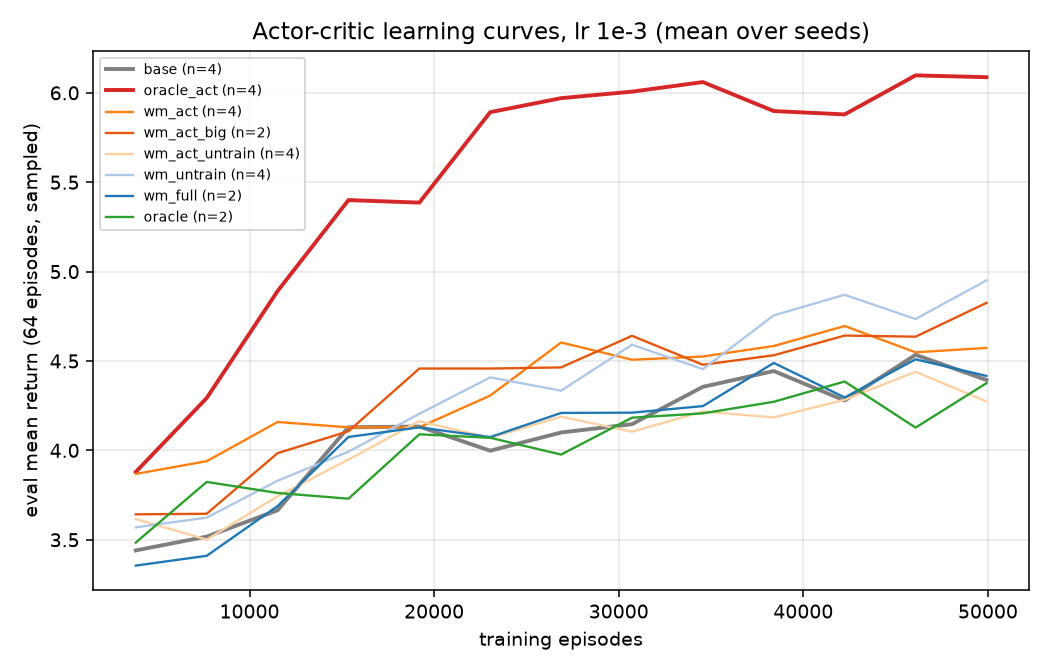
\includegraphics[width=0.75\textwidth]{res_ac_curves.png}
\caption{Learning curves of the 49.9k-episode runs (mean over seeds; evaluation of 64 episodes every 60 updates). Source: \srcpath{output/arc\_proposals/ac\_stageb\_long/}, \srcpath{ac\_long*/}, \srcpath{ac\_actreward\_*/}.}
\end{figure}

\subsection{Derivative: a learned (deployable) version of the \texttt{oracle\_act} signal}
\texttt{oracle\_act} needs the simulator at policy time. We trained an MLP (2$\times$512, GELU) that maps the raw 1345-d observation to the 17 one-step rewards, with labels from simulator branching used only offline (random-policy episodes, 80/20 split by episode), and served its predictions in the same 17 feature slots (arm \texttt{wm\_act}; \texttt{wm\_act\_untrain} = same network with random weights).
\begin{table}[h]
\centering\small
\caption{Held-out quality of the learned action-reward model. ``Action-dependent'' = the part of the reward that differs between actions in a state (about 18--21\% of states).}
\begin{tabular}{lrr}
\toprule
& small (256 episodes) & big (1024 episodes) \\
\midrule
train states / test states & 27{,}187 / 7{,}951 & 116{,}978 / 28{,}716 \\
$R^2$ over all 17 outputs & 0.548 & 0.633 \\
$R^2$ of the action-dependent part & 0.487 & 0.620 \\
best-action hit rate on action-dependent states & 86.4\% & 87.3\% \\
\quad uniform random / always the globally best action & 12.3\% / 64.3\% & 14.9\% / 61.8\% \\
\bottomrule
\end{tabular}
\end{table}

\begin{table}[h]
\centering\small
\caption{Actor-critic with the learned action-reward features, lr $10^{-3}$.}
\begin{tabular}{lp{5.2cm}p{5.2cm}}
\toprule
arm & 12.8k episodes & 49.9k episodes \\
\midrule
\texttt{base} & $3.47\pm0.07$ (n=8) & $4.36\pm0.16$ (4) \\
\texttt{wm\_act\_untrain} (control) & $3.52\pm0.08$ (8) & $4.30\pm0.09$ (4) \\
\texttt{wm\_act} (small model) & $\mathbf{3.75\pm0.18}$ (8); $+0.28$ vs.\ base (p=.002), $+0.23$ vs.\ control (p=.009) & $4.49\pm0.14$ (4); $+0.13$ (p=.25) \\
\texttt{wm\_act} (big model) & $3.78\pm0.10$ (4); $+0.31$ (p=.003) & $4.61\pm0.03$ (2); $+0.25$ (p=.04, n=2) \\
\texttt{oracle\_act} (leaked) & $4.49\pm0.26$ (6) & $6.13\pm0.17$ (4) \\
\bottomrule
\end{tabular}
\end{table}
The learned signal is a real but small improvement: about a quarter of the leaked gain at 12.8k episodes ($+0.28$ of $+1.03$) and about 7--14\% at 49.9k episodes ($+0.13$ to $+0.25$ of $+1.78$, not clearly significant). The larger model, despite better held-out $R^2$, gives about the same policy result at 12.8k episodes.

\section{ChunkPPO with $\delta>0$}

\subsection{What we did}
The existing chunk-level PPO (\srcpath{src/pipeline/chunk\_ppo.py}, unchanged) on two latency environments, driven by a new script that exposes every config field (\srcpath{scripts/run\_latency\_sweep2.py}):
\begin{itemize}
\item \texttt{intercept}: unit arena, exogenous randomly turning target; catching gives $+1$ and ends the episode, 1 cost per step; 5 discrete moves; 200 ticks.
\item \texttt{pendulum\_goal}: torque-limited pendulum (5 torques) with a goal angle; 200 ticks.
\end{itemize}
Chunk length $k=8$, latency $\delta\in\{0,1,2,4,8\}$ ticks (at $\delta=0$ only \texttt{augment} is run; all arms see the same state there). Arms differ only in the actor's input: \texttt{ignore} (snapshot only), \texttt{augment} (snapshot + committed prefix $u_c$), \texttt{wm} (factored world-model forecast of the state at $t_c+\delta$ from $(o_c,u_c)$, co-trained, with 12{,}800 passive reference-action ticks charged to its budget), \texttt{wm\_passive} (forecast that ignores the committed actions; the original ``noop model'' proposal), \texttt{oracle} (exact future state including future noise; upper bound that no causal agent can reach). The critic, optimiser, budget and architecture are the same in all arms. Metric: \texttt{eval\_return} = mean return of the first episode of each of 64 fresh environments under the stochastic policy (protocol v2).

\paragraph{Learner configurations.} The pre-registered default (64 envs $\times$ 32 cycles $\times$ $k$ = 16{,}384 ticks/update, lr $3\cdot10^{-4}$, 1M ticks $\Rightarrow$ about 61 PPO updates) learns \texttt{intercept} ($\delta=0$ return 0.58) but does not learn \texttt{pendulum\_goal} (return $-178$ at $\delta=0$, about $-180$ for every arm and $\delta$; 1 seed). Pilots at $\delta=0$, 2M ticks: config A (16 envs $\times$ 16 cycles = 2048 ticks/update, lr $10^{-3}$) reached 0.70 on \texttt{intercept} and $-63$ on \texttt{pendulum\_goal}; config B (32 envs $\times$ 16 cycles, lr $3\cdot10^{-4}$, entropy 0.003) reached 0.72 and $-85$. Config A was used for the main sweeps; config B was then run on \texttt{intercept} as a robustness check.

\subsection{Results: intercept}
\begin{figure}[h]
\centering
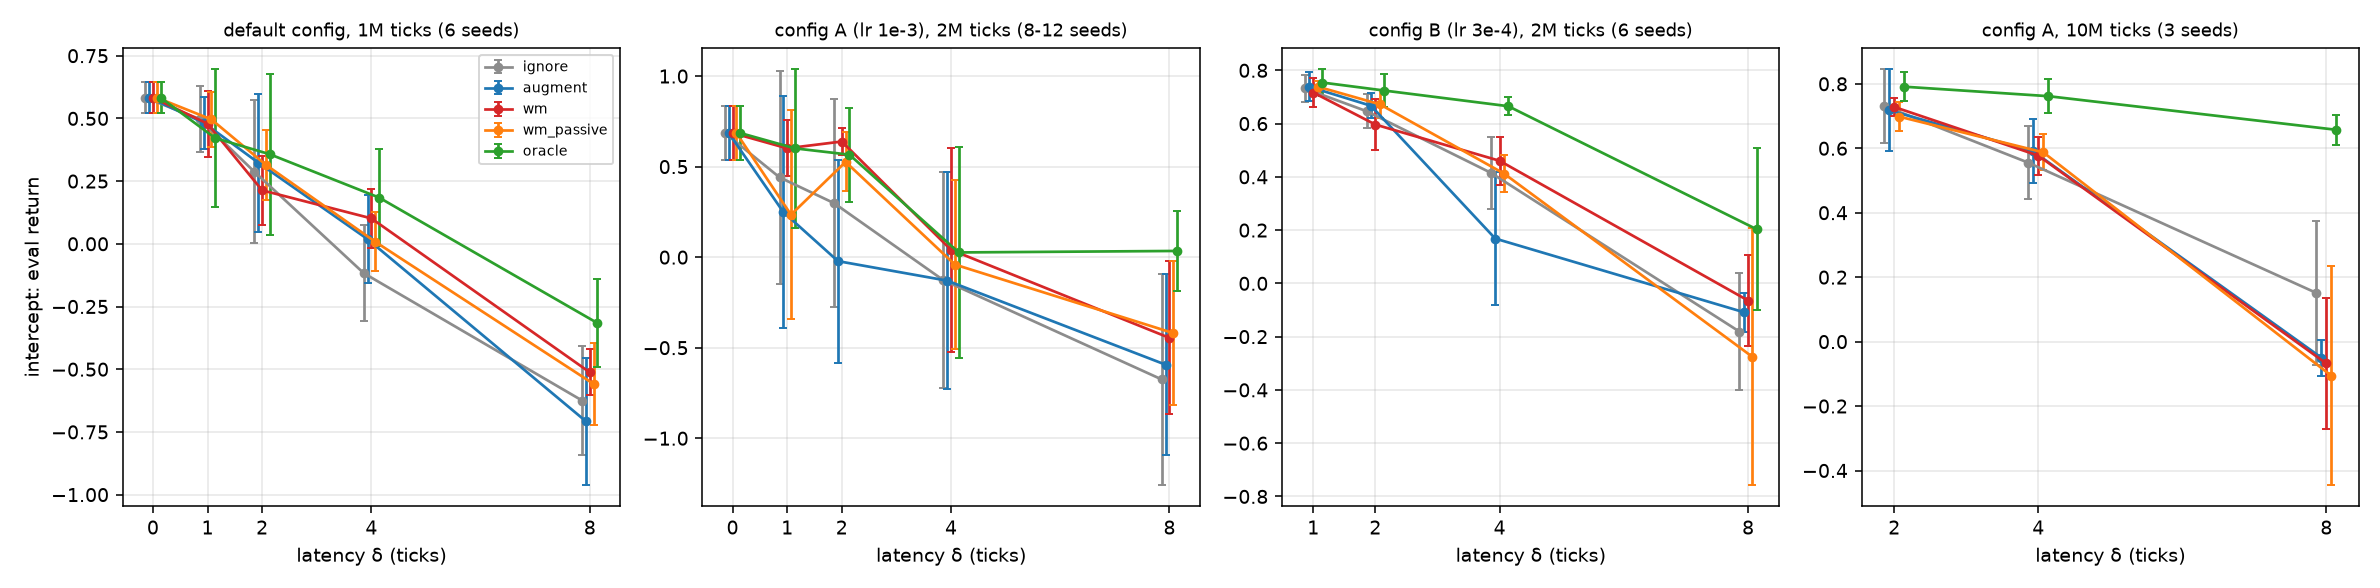
\includegraphics[width=\textwidth]{res_latency_intercept.png}
\caption{Intercept: evaluation return vs.\ latency $\delta$ for the five arms (mean $\pm$ sd over seeds). From left: default config at 1M ticks; config A at 2M ticks (8 seeds, 12 at $\delta=2,4$); config B at 2M ticks (6 seeds); config A at 10M ticks (3 seeds). Source: \srcpath{output/arc\_proposals/latency/}.}
\end{figure}

\begin{table}[h]
\centering\small
\caption{Intercept, evaluation return (mean $\pm$ sd). $n$: A = 8 (12 at $\delta=2,4$), B = 6, 10M = 3, default = 6.}
\begin{tabular}{llrrrrr}
\toprule
setting & $\delta$ & ignore & augment & wm & wm\_passive & oracle \\
\midrule
A, 2M ticks & 0 & & $.69\pm.15$ & & & \\
& 1 & $.44\pm.59$ & $.25\pm.64$ & $.60\pm.15$ & $.23\pm.58$ & $.60\pm.44$ \\
& 2 & $.30\pm.58$ & $-.02\pm.56$ & $\mathbf{.64\pm.08}$ & $.53\pm.16$ & $.57\pm.26$ \\
& 4 & $-.13\pm.60$ & $-.13\pm.60$ & $.04\pm.56$ & $-.04\pm.47$ & $.03\pm.58$ \\
& 8 & $-.68\pm.58$ & $-.59\pm.50$ & $-.45\pm.42$ & $-.42\pm.40$ & $.03\pm.22$ \\
\midrule
B, 2M ticks & 1 & $.73\pm.05$ & $.74\pm.06$ & $.72\pm.06$ & $.74\pm.02$ & $.75\pm.05$ \\
& 2 & $.65\pm.06$ & $.67\pm.05$ & $.60\pm.09$ & $.67\pm.05$ & $.72\pm.06$ \\
& 4 & $.42\pm.13$ & $.17\pm.25$ & $\mathbf{.46\pm.09}$ & $.41\pm.07$ & $.67\pm.03$ \\
& 8 & $-.18\pm.22$ & $-.11\pm.07$ & $-.06\pm.17$ & $-.28\pm.48$ & $.20\pm.30$ \\
\midrule
A, 10M ticks & 2 & $.73\pm.12$ & $.72\pm.13$ & $.73\pm.03$ & $.70\pm.04$ & $.79\pm.04$ \\
& 4 & $.56\pm.11$ & $.59\pm.10$ & $.58\pm.06$ & $.59\pm.06$ & $.76\pm.05$ \\
& 8 & $.15\pm.22$ & $-.05\pm.06$ & $-.07\pm.20$ & $-.11\pm.34$ & $.66\pm.05$ \\
\midrule
default, 1M ticks & 0 & & $.58\pm.06$ & & & \\
& 1 & $.50\pm.13$ & $.48\pm.10$ & $.48\pm.13$ & $.50\pm.11$ & $.42\pm.28$ \\
& 2 & $.29\pm.29$ & $.32\pm.28$ & $.21\pm.14$ & $.31\pm.14$ & $.36\pm.32$ \\
& 4 & $-.12\pm.19$ & $.02\pm.17$ & $.10\pm.12$ & $.01\pm.12$ & $.18\pm.19$ \\
& 8 & $-.63\pm.22$ & $-.71\pm.25$ & $-.51\pm.09$ & $-.56\pm.16$ & $-.32\pm.18$ \\
\bottomrule
\end{tabular}
\end{table}

Permutation tests against \texttt{augment} (same setting and $\delta$):
\begin{itemize}
\item Config A, $\delta=2$ (12 seeds): \texttt{wm} $+0.66$ (p$<0.001$; 12/12 seeds above 0.4 vs.\ 4/12 for \texttt{augment}), \texttt{wm\_passive} $+0.55$ (p=0.004), \texttt{oracle} $+0.59$ (p=0.004). Config A, $\delta=1,4,8$ (8/12/8 seeds): \texttt{wm} $+0.35$, $+0.17$, $+0.15$, none significant; \texttt{oracle} significant only at $\delta=8$ ($+0.63$, p=0.005).
\item Config B, $\delta=2$: \texttt{wm} $-0.07$ (p=0.14), i.e.\ the gap is gone (\texttt{augment} 0.67 vs.\ 0.03 under config A). $\delta=4$: \texttt{wm} $+0.29$ (p=0.02), but \texttt{ignore} $+0.25$ (p=0.049) and \texttt{wm\_passive} $+0.24$ (p=0.04) show the same gain, and \texttt{wm}$-$\texttt{ignore} $=+0.04$. $\delta=1,8$: nothing significant except \texttt{oracle} at $\delta=8$ ($+0.31$, p=0.05).
\item 10M ticks: all causal arms are equal within noise at $\delta=2$ (0.70--0.73) and $\delta=4$ (0.56--0.59); \texttt{oracle} stays higher at $\delta=4$ and 8 because it sees the target's future random turns.
\item \texttt{augment} vs.\ \texttt{ignore}: never significantly better in any setting; significantly worse only for config B at $\delta=4$.
\end{itemize}
The cost of latency itself is clear: the best causal return falls from about 0.7--0.8 at $\delta=0$ to about 0.7 at $\delta=1$--2, about 0.5--0.6 at $\delta=4$ and about 0--0.15 at $\delta=8$.

\subsection{Results: pendulum\_goal}
\begin{figure}[h]
\centering
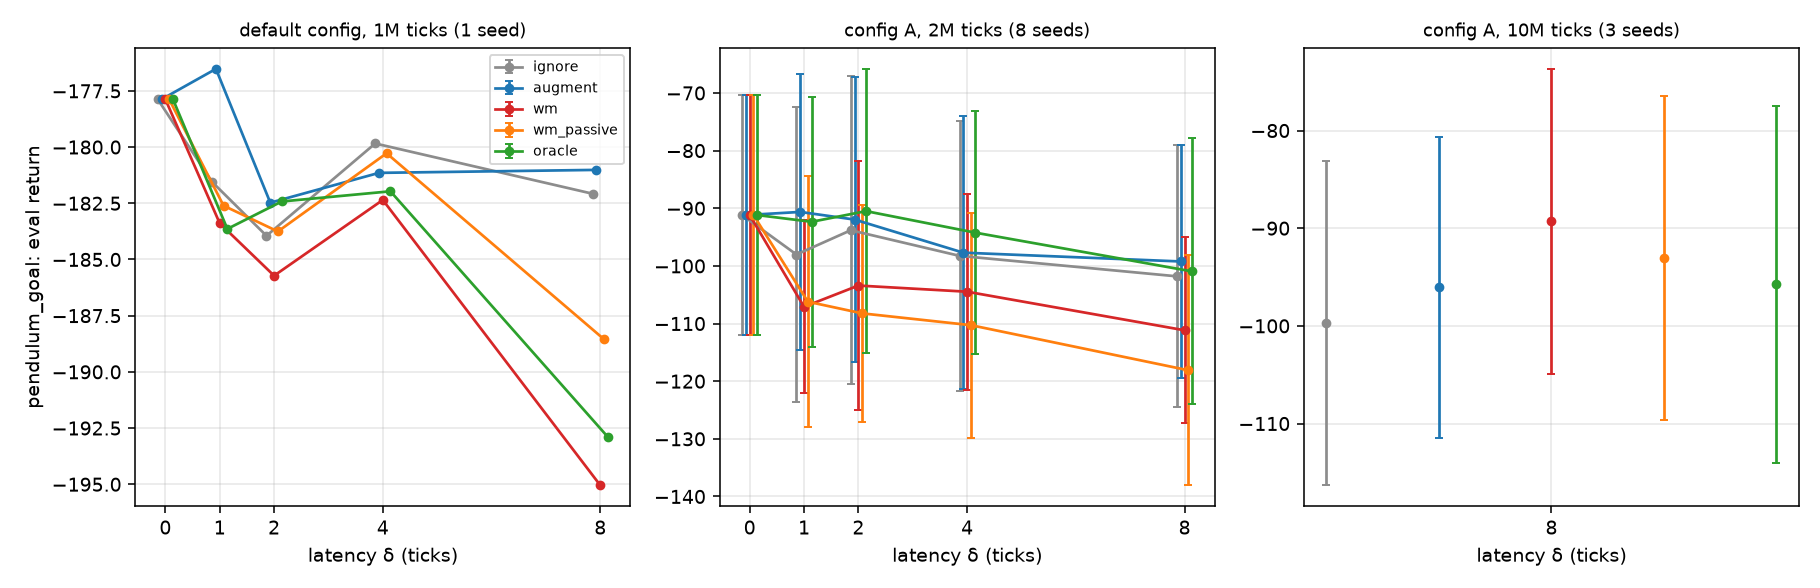
\includegraphics[width=0.85\textwidth]{res_latency_pendulum.png}
\caption{pendulum\_goal: evaluation return vs.\ $\delta$. Left: default config at 1M ticks (1 seed; no learning). Middle: config A at 2M ticks (8 seeds). Right: config A at 10M ticks, $\delta=8$ only (3 seeds). Source: \srcpath{output/arc\_proposals/latency/}.}
\end{figure}

\begin{table}[h]
\centering\small
\caption{pendulum\_goal, config A, 2M ticks, 8 seeds (mean $\pm$ sd).}
\begin{tabular}{lrrrrr}
\toprule
$\delta$ & ignore & augment & wm & wm\_passive & oracle \\
\midrule
0 & & $-91.2\pm20.8$ & & & \\
1 & $-98.0\pm25.7$ & $-90.6\pm23.9$ & $-107.1\pm15.0$ & $-106.2\pm21.8$ & $-92.4\pm21.7$ \\
2 & $-93.8\pm26.7$ & $-92.0\pm24.8$ & $-103.4\pm21.5$ & $-108.2\pm18.8$ & $-90.5\pm24.7$ \\
4 & $-98.3\pm23.4$ & $-97.7\pm23.7$ & $-104.5\pm17.0$ & $-110.3\pm19.5$ & $-94.2\pm21.1$ \\
8 & $-101.8\pm22.7$ & $-99.2\pm20.2$ & $-111.2\pm16.1$ & $-118.1\pm20.0$ & $-101.0\pm23.1$ \\
\midrule
8 (10M ticks, 3 seeds) & $-99.7\pm16.6$ & $-96.1\pm15.4$ & $-89.3\pm15.6$ & $-93.1\pm16.6$ & $-95.7\pm18.3$ \\
\bottomrule
\end{tabular}
\end{table}
On \texttt{pendulum\_goal} the forecast arms are $-7$ to $-16$ below \texttt{augment} at 2M ticks (none significant, p between 0.12 and 0.52 for \texttt{wm}) and \texttt{augment}, \texttt{ignore} and \texttt{oracle} are indistinguishable, i.e.\ latency up to $\delta=8$ costs only a few return units here. At 10M ticks all arms are within one sd of each other.

\section{Overall reading}
\begin{itemize}
\item \textbf{Structure-as-input}: useful as an input feature where the network must extrapolate beyond its data, but on this testbed the benefit is provided by any unbounded monotone feature; hard-coding a wrong formula is harmful; a route chosen by ID error cannot detect OOD failure.
\item \textbf{Actor-critic}: under PPO+GAE+critic (lr $\ge10^{-3}$) the \texttt{oracle\_act} litmus passes clearly, which the REINFORCE learner could not show. The noop-anticipation world model is not useful (even its oracle version); the learned action-reward model recovers part of the leaked gain at the smaller budget.
\item \textbf{ChunkPPO $\delta>0$}: the forecast arms show no gain that survives a change of learner configuration or a larger budget; the visible gaps come from \texttt{augment} failing to optimise at one particular $\delta$.
\end{itemize}

\end{document}
